%\documentclass[handout,xcolor=pdftex,dvipsnames,table,mathserif]{beamer} 
\documentclass[xcolor=pdftex,dvipsnames,table]{beamer}
%\usepackage{subfigure}
\usepackage{amsbsy}
\usepackage{tikz}
\usetikzlibrary{arrows}
\usepackage{amsmath,graphicx,dsfont,color}
\usepackage{amsfonts}
\usepackage{amssymb}
\usepackage{array}

\usepackage{subfig}

% makes the subfig package work
\makeatletter
\let\@@magyar@captionfix\relax
\makeatother

% subfigure counter resets every frame
\makeatletter
\@addtoreset{subfigure}{framenumber}
\makeatother

% First author and year
\bibliographystyle{apalike}

% This sets the list items of the bibliography to the same symbol used for citation.
\setbeamertemplate{bibliography item}{\insertbiblabel}

% This avoids extralines for different entries
\setbeamertemplate{bibliography entry title}{}
\setbeamertemplate{bibliography entry location}{}
\setbeamertemplate{bibliography entry note}{}

\DeclareMathOperator*{\argmin}{arg\,min}
\DeclareMathOperator*{\argmax}{arg\,max}
%Definitiona

\newcommand{\x}{\mathbf{x}}
\newcommand{\X}{\mathbf{X}}
\newcommand{\W}{\mathbf{W}} %Weight
\newcommand{\bais}{\mathbf{b}}%Bais
\newcommand{\act}{\texttt{g}}%Activation
\newcommand{\loss}{L}
\newcommand{\pdata}{\hat{p}_{\texttt{data}}}
\newcommand{\nsize}{N}
\newcommand{\nfeatures}{P}
\newcommand{\param}{\boldsymbol{\theta}}
\newcommand{\featmap}{\boldsymbol{\phi}}
\newcommand{\EV}{\mathbb{E}}









\title{Deep Learning for Image Analysis - \\ 
	   Visualization of Neural Networks}
\author{Thomas Walter, PhD}
\date{Centre for Computational Biology (CBIO) \\
	  MINES Paris-Tech, PSL Research University \\
	  Institut Curie, PSL Research University \\
	  INSERM U900}


%To include LOGO?
%\logo{\includegraphics[width=.1\columnwidth]{MinesLogo}}
\useinnertheme{rounded}
\usecolortheme{rose}

\usepackage{xcolor}
\definecolor{lightblue}{RGB}{0,200,255}


\setbeamertemplate{footline}[frame number]{}
\setbeamertemplate{navigation symbols}{}
\setbeamertemplate{section in toc}[square]
\setbeamertemplate{items}[square]

%% For image credits on image bottom right
\usepackage[absolute,overlay]{textpos}
\setbeamercolor{framesource}{fg=gray}
\setbeamerfont{framesource}{size=\tiny}
\newcommand{\source}[1]{\begin{textblock*}{4cm}(8.7cm,8.6cm)
    \begin{beamercolorbox}[ht=0.5cm,right]{framesource}
      \usebeamerfont{framesource}\usebeamercolor[fg]{framesource} Credits: {#1}
    \end{beamercolorbox}
\end{textblock*}}


\begin{document}

\begin{frame}
\titlepage
\end{frame}

\begin{frame}{Overview}
\tableofcontents
\end{frame}

%%%%%%%%%%%%%%%%%%%%%%%%%%%%%%%%%%%%%%%%%%%%%%%%%%%%%%%%%%%%%%%%%%%%%%%%%
%%%%%%%%%%%%%%%%%%%%%%%%%%%%%%%%%%%%%%%%%%%%%%%%%%%%%%%%%%%%%%%%%%%%%%%%%
\section{Introduction}

% \subsection{Motivation: visualization and understanding}
\begin{frame}{Motivation: visualization and understanding}
	\begin{itemize}
		\item Convolutional Neural Networks have achieved stunning performance for many tasks, such as image classification, image segmentation and object detection. 
		\item CNN can be difficult to train, and results can be very variable for different settings of hyperparameters. 
		\item It is unclear, how design choices (network architecture, initialization, weight decay, $\ldots$) effect trainability and performance. 
		\item It is not very well understood what Neural Networks actually learn. 
		\item One idea to approach some of these issues relies on {\bf visualization}.
	\end{itemize}
\end{frame}

% \subsection{Categorization}
% \begin{frame}{Categorization of visualization approaches}
% 	\begin{itemize}
% 		\item Image-dependent visualizations
% 		\item Image-independent visualizations
% 	\end{itemize}
% \end{frame}

%%%%%%%%%%%%%%%%%%%%%%%%%%%%%%%%%%%%%%%%%%%%%%%%%%%%%%%%%%%%%%%%%%%%%%%%%
%%%%%%%%%%%%%%%%%%%%%%%%%%%%%%%%%%%%%%%%%%%%%%%%%%%%%%%%%%%%%%%%%%%%%%%%%
\section{Visualization of filters}
\frame{\frametitle{Overview}\tableofcontents[currentsection]}

\begin{frame}{Filters in Neural Networks}
\begin{figure}[htb]
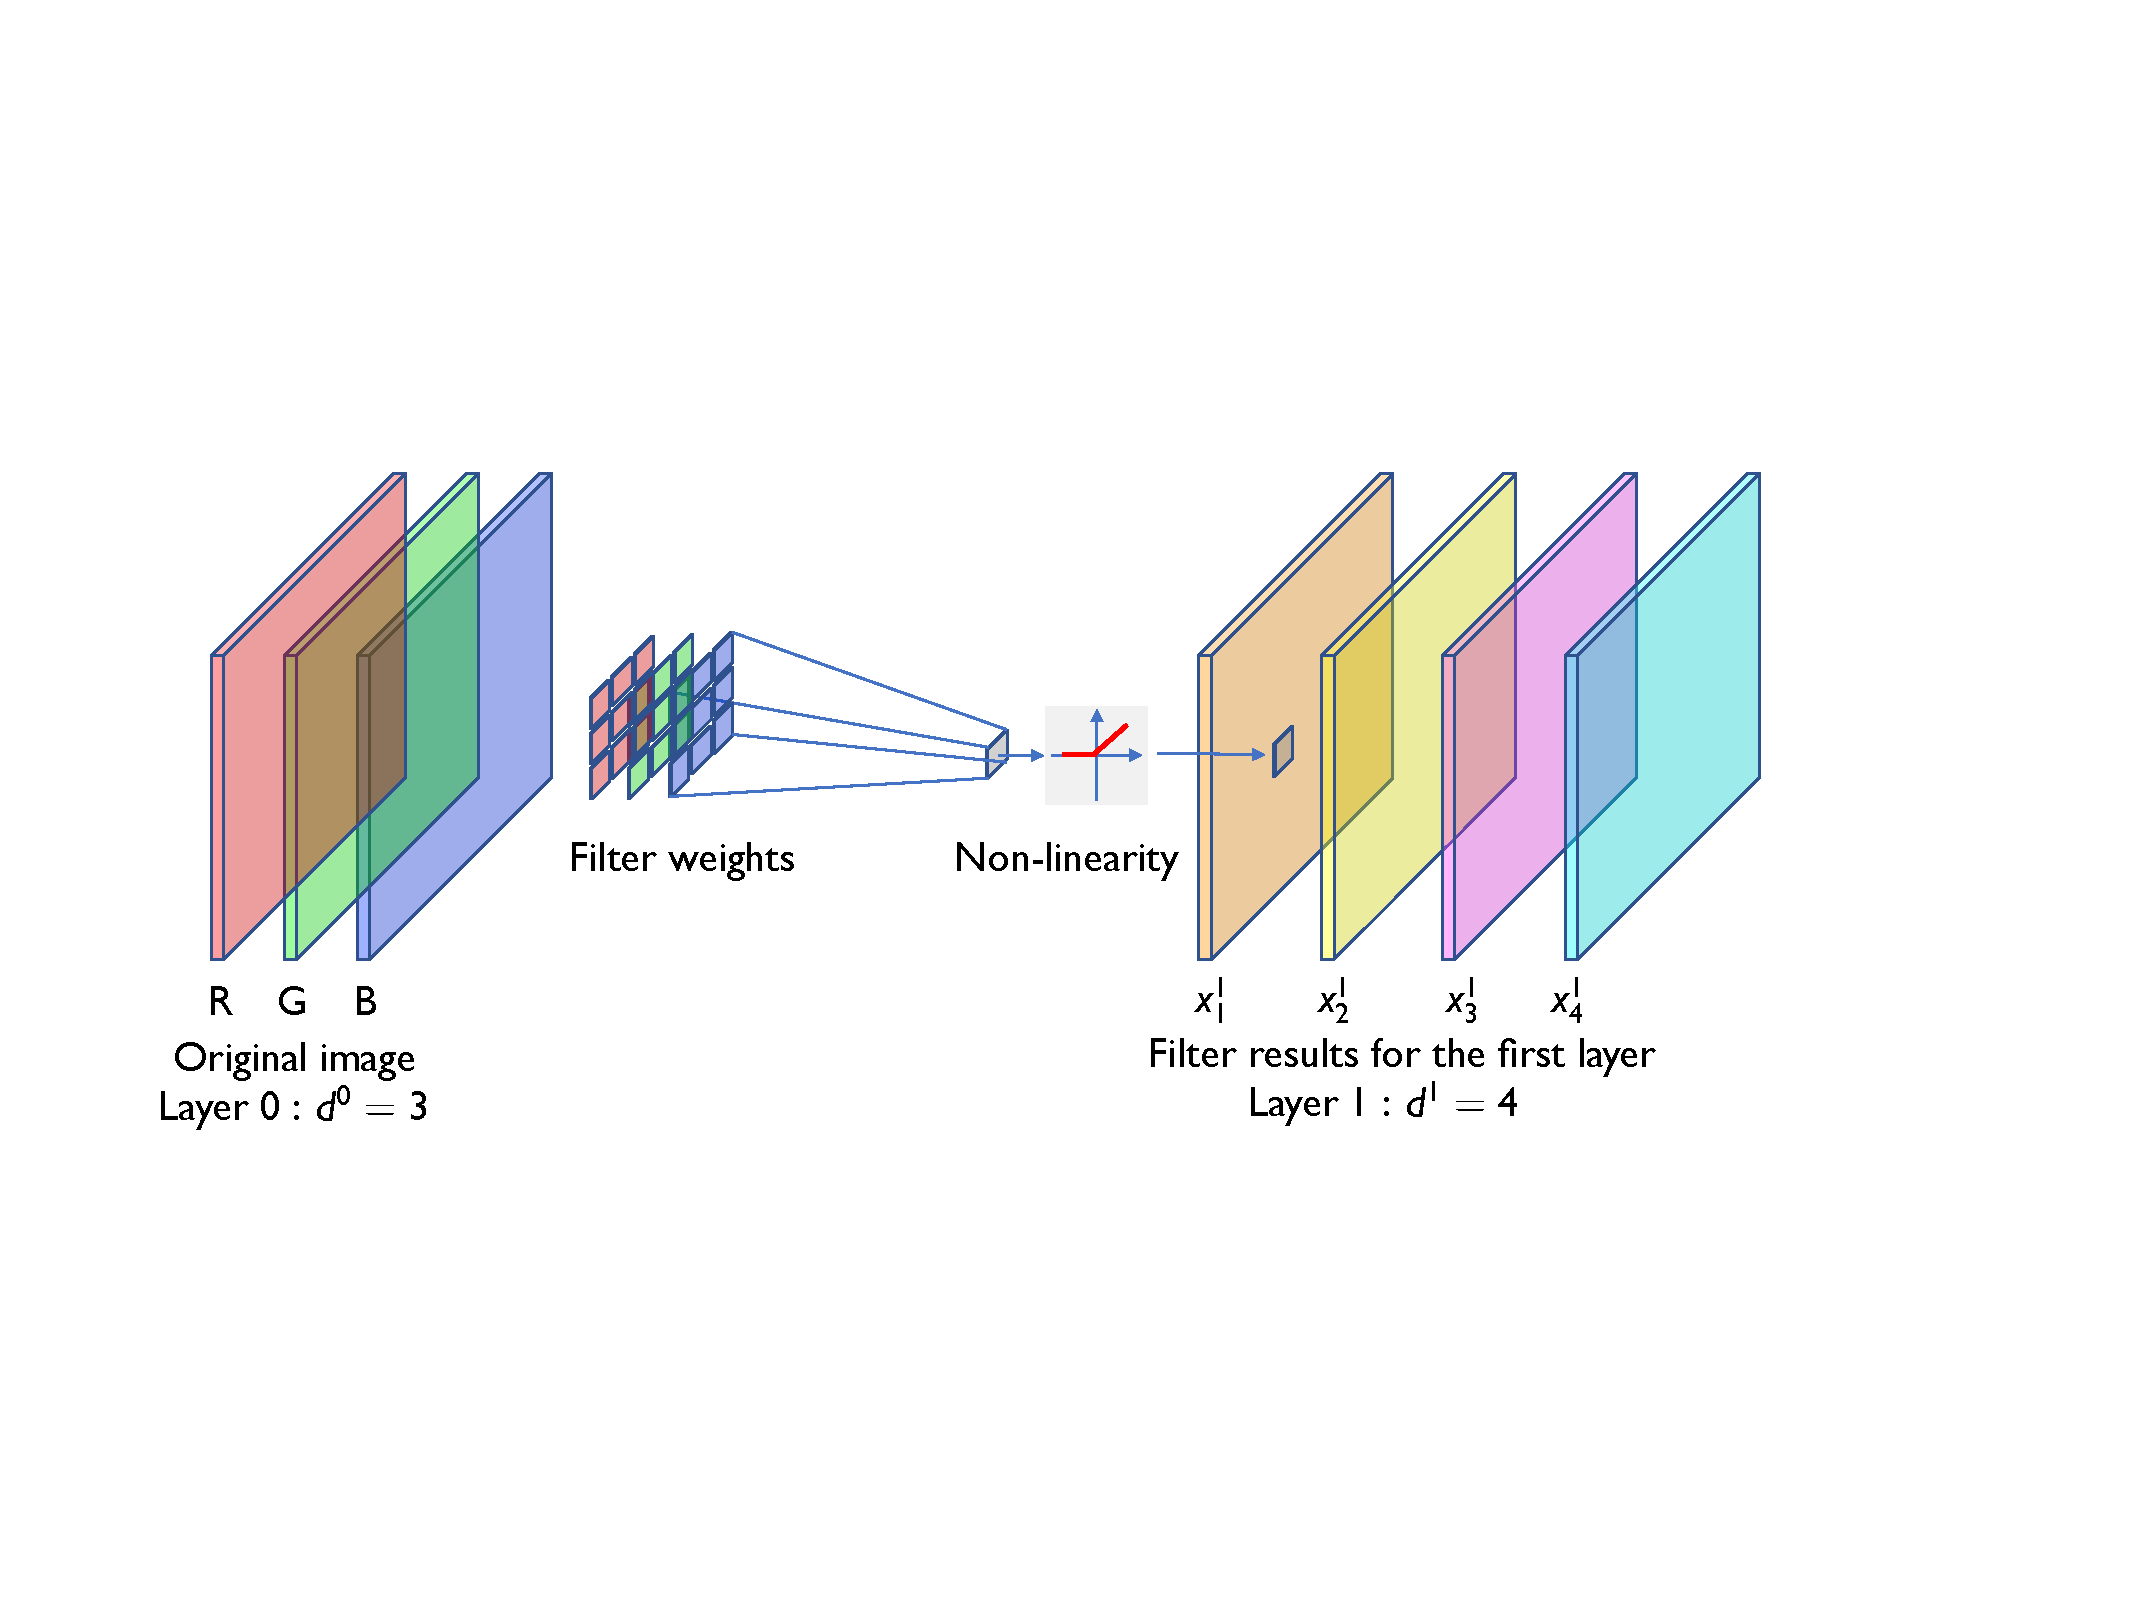
\includegraphics[width=0.9\textwidth]{../graphics/CNN_FirstLayer.pdf}
\end{figure}
In Convolutional Neural Networks (CNN), a pixel value in activation map $r$ in layer $l$ depends on the pixel values in layer $l-1$ within the receptive field of the filter $W^{l}_r$ across all channels. The pixel value $x^{l}_{r}(n,m)$ at position $n,m$ in the activation map $r$ in layer $l$ is\footnote{For simplicity, we do not consider downsampling operations and to not consider border effects}: 
\begin{equation}
	x^{l}_{r}(n,m) = g(\sum_k\sum_{i,j}W^{l}_r(i,j,k)x^{l-1}_{k}(n+i,m+j) + b^l_r)
\end{equation} 
\end{frame}

\begin{frame}{Filters in Neural Networks}
\begin{figure}[htb]
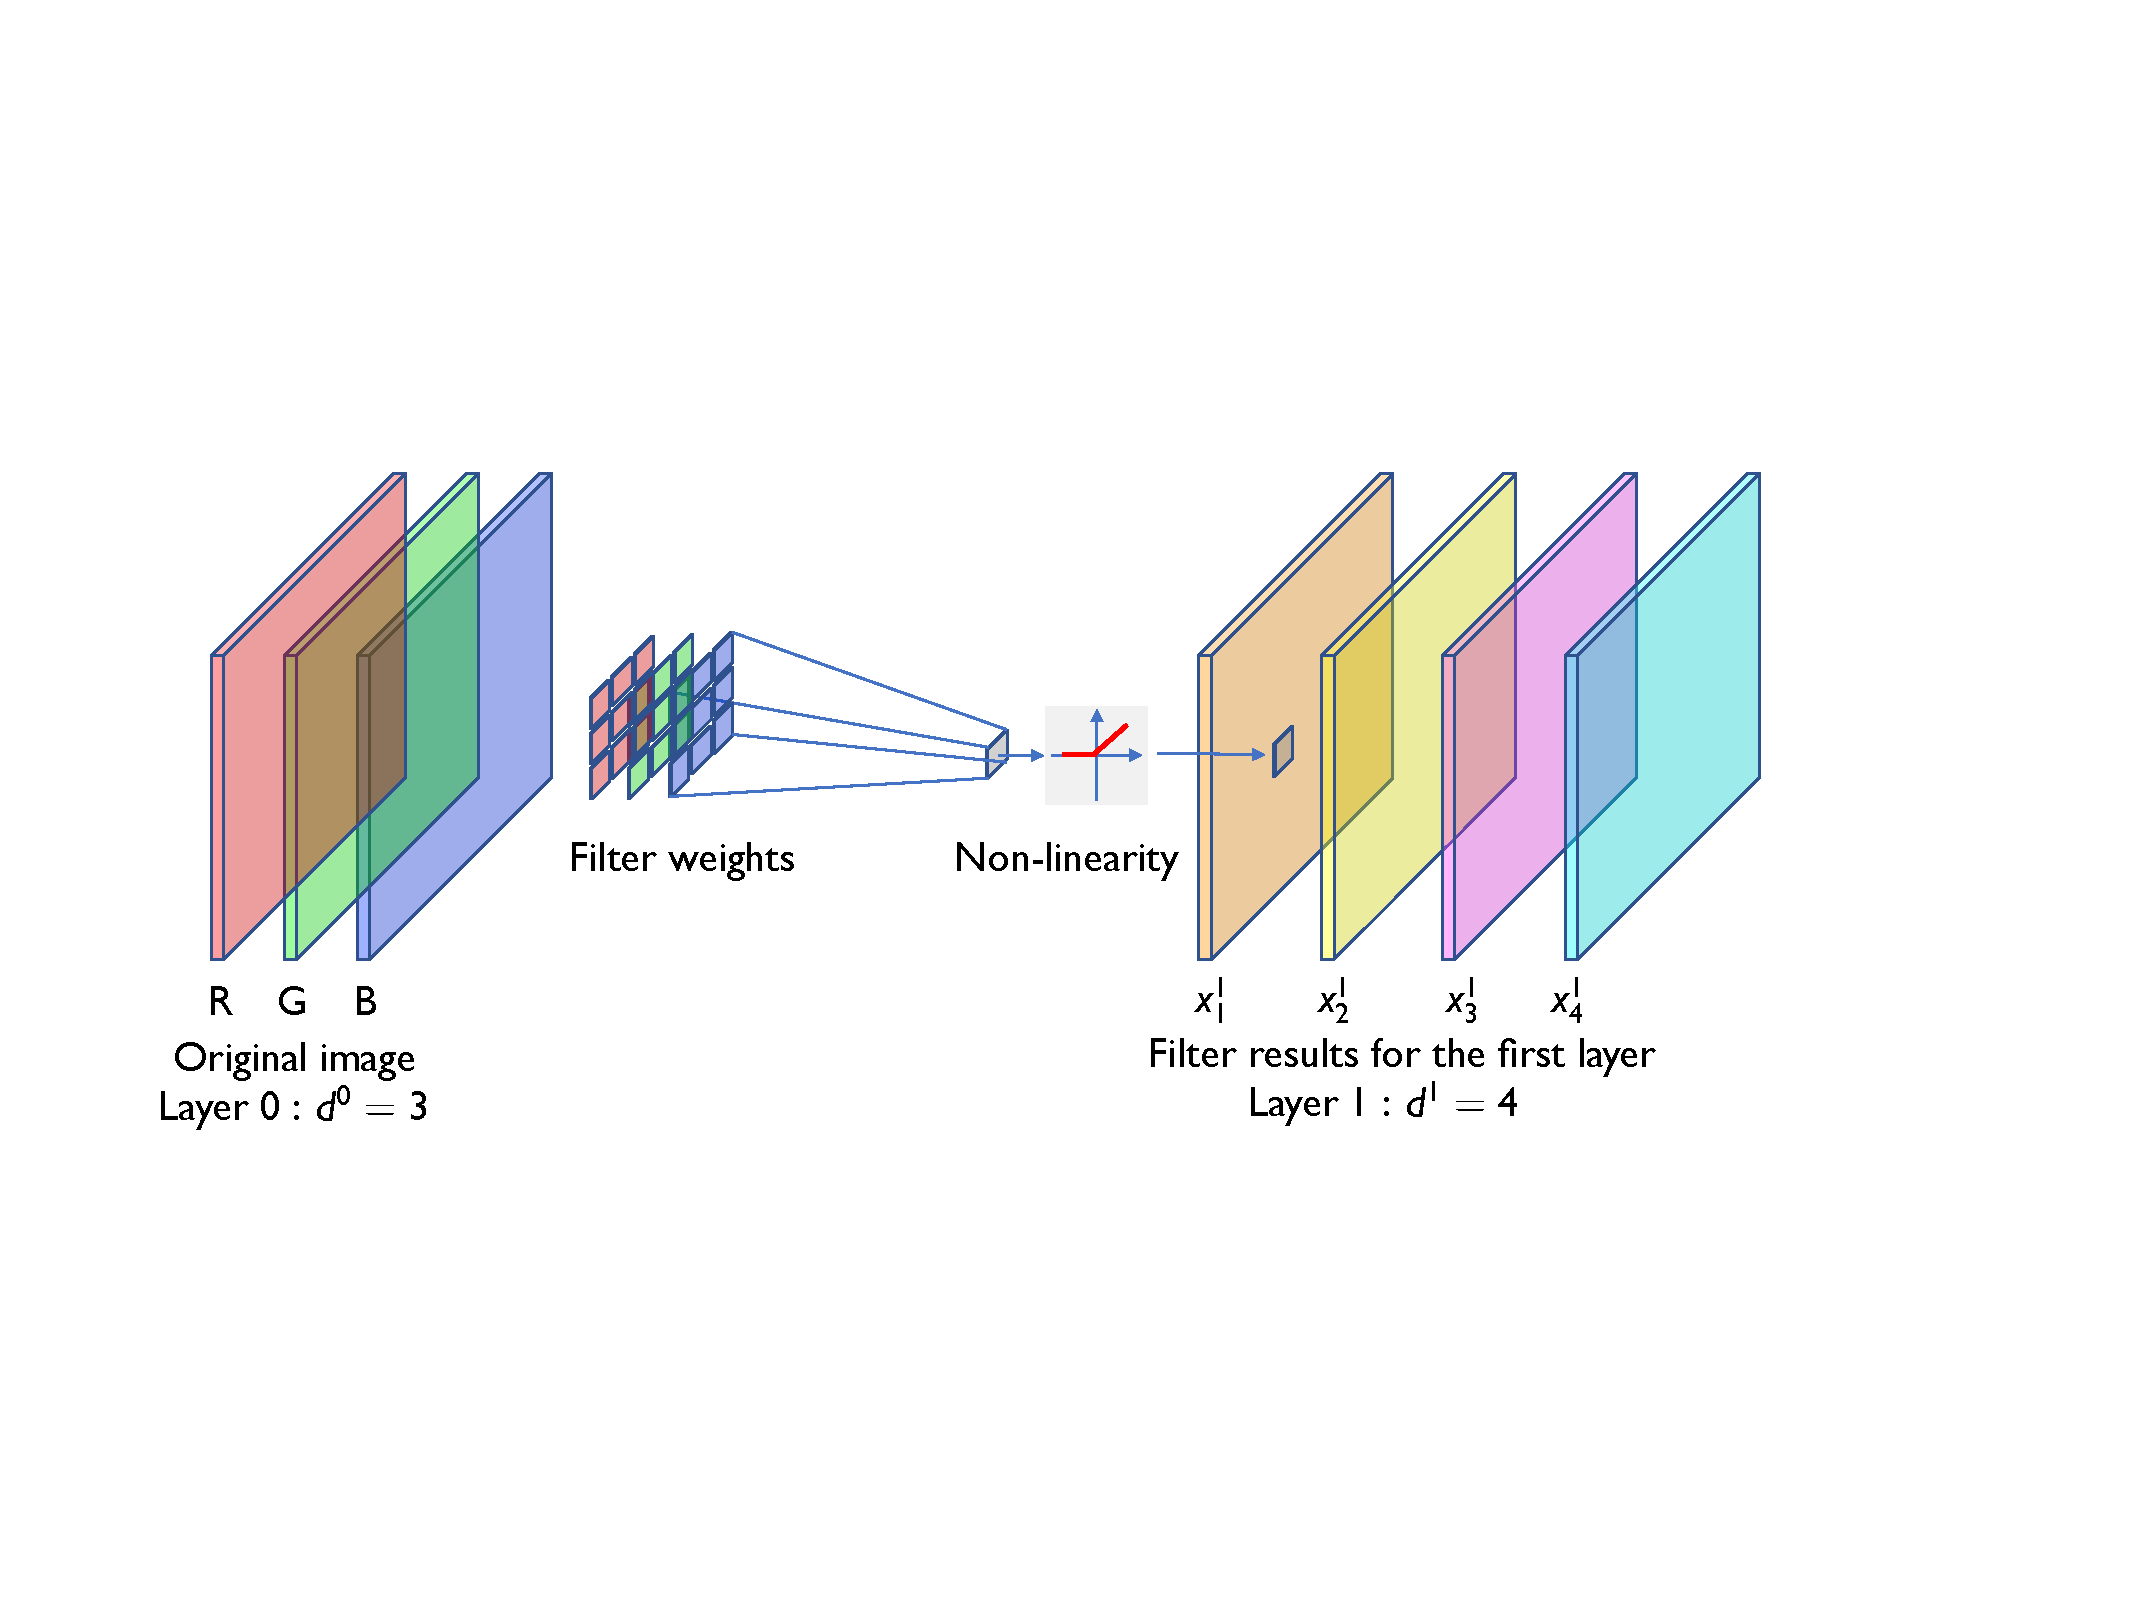
\includegraphics[width=0.9\textwidth]{../graphics/CNN_FirstLayer.pdf}
\end{figure}
\begin{itemize}
	\item Each filter $W^l_r$ (filter $r$ in layer $l$) is thus a 3D tensor of values with dimension $d^{l-1}\times s^l\times s^l$.
	\item For the first layer, the number of input channels is typically 3, i.e. for each pixel, there are 3 values available ($R$, $G$ and $B$).  
	\item For this reason, all filters of layer 1 have the dimension $3\times s^{1}\times s^{1}$. 
	\item This means that each filter corresponds itself to an $RGB$ image of size $s^{1}\times s^{1}$. 
\end{itemize}
\end{frame}

\begin{frame}{Visualization of the first layer filters}
\begin{figure}[htb]
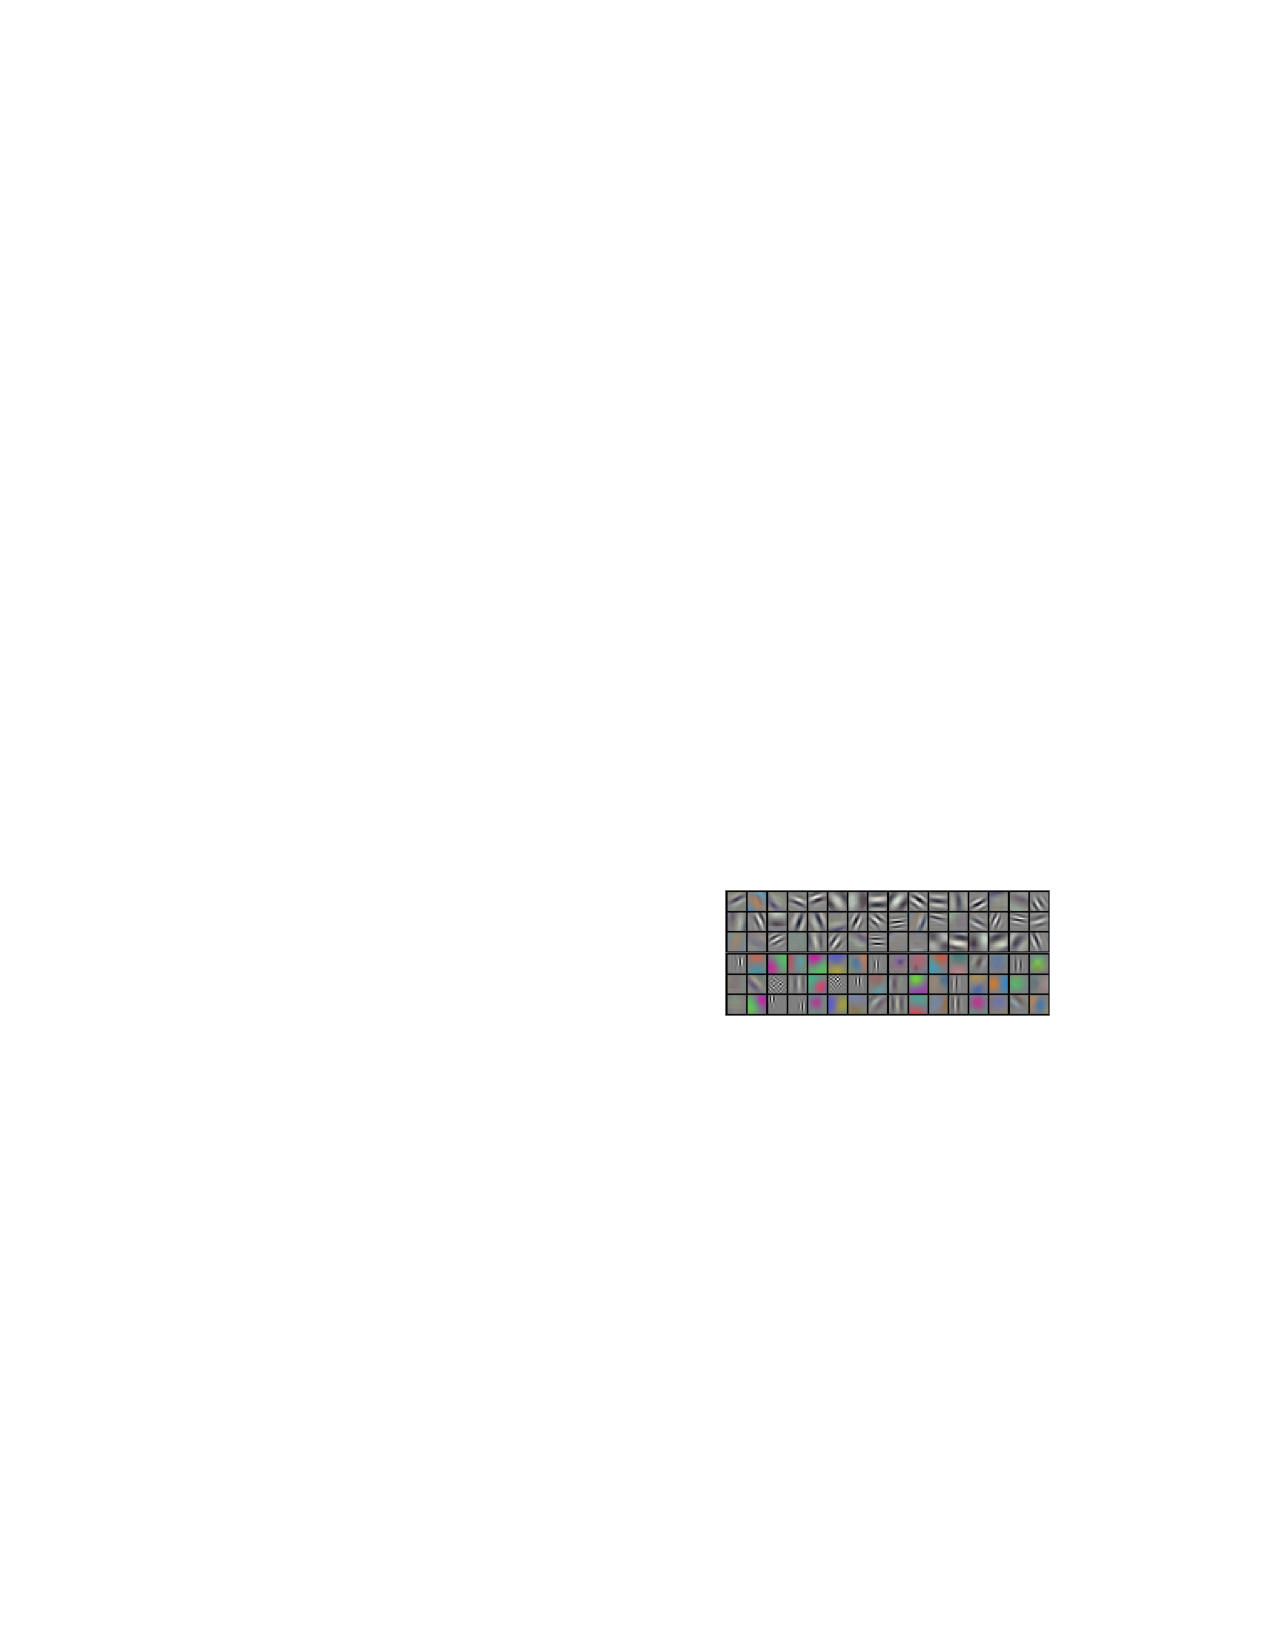
\includegraphics[width=0.9\textwidth]{../graphics/Vis_filter_imagenet.pdf}
\end{figure}
\begin{itemize}
	\item First layer filters obtained by the Alexnet in the Imagenet competition \cite{Krizhevsky:2012}. 
	\item Observation: they contain oriented contours (top row) and color blobs (bottom row). 
	\item How can we interpret this? 
\end{itemize}
\end{frame}

\begin{frame}{Visualization of first layer filters}
\begin{itemize}
	\item The scalar product $w^Tx$ is maximal if $x$ points into the same direction as $w$:
	\begin{equation*}
	w^Tx = \|w\|\|x\|\cos{\alpha_{x,w}}
	\end{equation*}
	\item Consequently the activation maps have high values, if the patterns in the image coincide with the filters. 
	\item We therefore see, that the first layer of a trained convolutional neural network extracts low-level visual information, such as corners, edges, colors. 
	\item The filter visualization strategy is not really applicable to deeper layers: as the filters in deeper layers act on the outputs of the first layer activation maps, it is unclear how to interpret the patterns they might show.
\end{itemize}
\end{frame}

%%%%%%%%%%%%%%%%%%%%%%%%%%%%%%%%%%%%%%%%%%%%%%%%%%%%%%%%%%%%%%%%%%%%%%%%%
%%%%%%%%%%%%%%%%%%%%%%%%%%%%%%%%%%%%%%%%%%%%%%%%%%%%%%%%%%%%%%%%%%%%%%%%%
\section{Visualization of the loss function}
\frame{\frametitle{Overview}\tableofcontents[currentsection]}

\begin{frame}{Motivation: visualization of the loss function}
\begin{itemize}
	\item We have seen that training a Neural Networks corresponds to solving a minimization problem: 
	\begin{equation*}
		\param ^{\ast} = \argmin_{\param} \loss (\param) + \mathcal{R}(\param)
	\end{equation*}
	where $\param$ is the vector of all parameters, $\mathcal{R}(\param)$ a regularization term and $\loss (\param)$ the loss term calculated on the training data:
	\begin{equation*}
		\loss (\param) = \sum_{i=1}^N \loss_i (\param)
	\end{equation*}
	\item Visualization of the loss can give us a hint on how complicated this task really is. 
	\item Visualization can also allow us to compare different architectures or initialization schemes.
\end{itemize}
\end{frame}

%\begin{frame}{Spotting problems by visual inspection of the loss}
%\begin{itemize}
%\end{itemize}
%\end{frame}

\begin{frame}{Convexity}
\begin{figure}[htb]
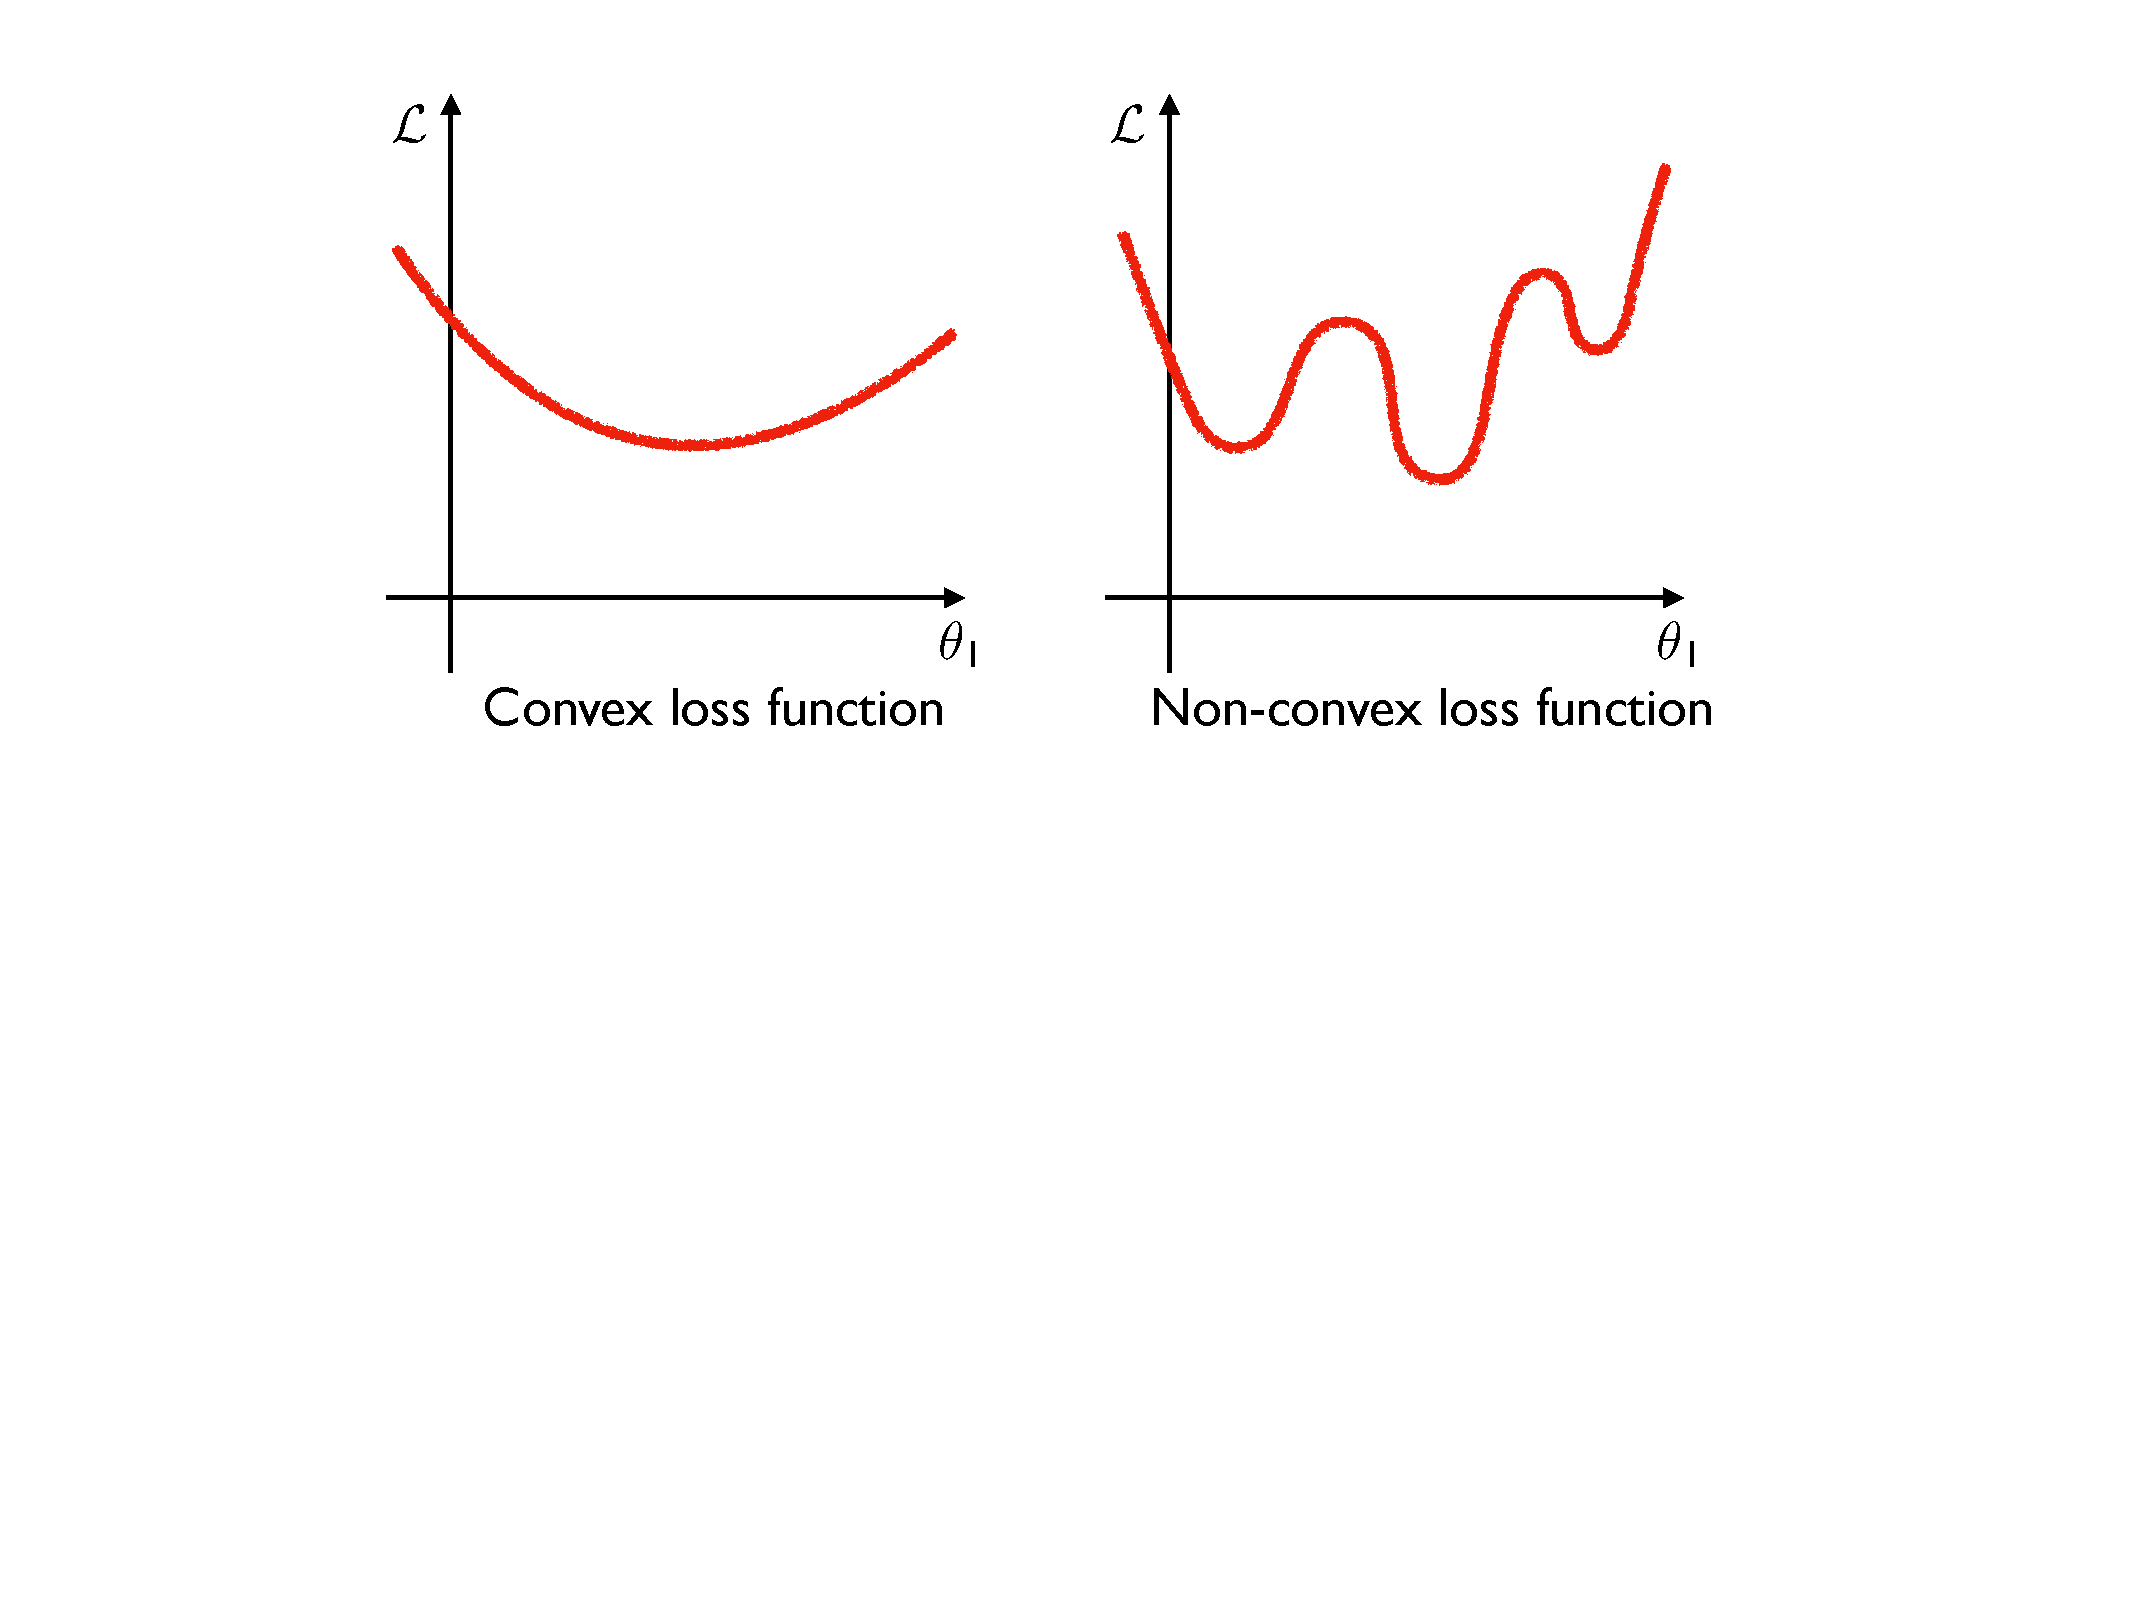
\includegraphics[width=0.9\textwidth]{../graphics/Vis_convexity.pdf}
\end{figure}
\begin{itemize}
	\item Convex optimization functions: only one local minimum (which is also the global minimum). 
	\item In neural networks, the loss is often not convex. 
	\item The shape of the loss is very important for the success of the optimization. 
	\item How can we visualize the loss w.r.t $\sim10^6$ parameters? 
\end{itemize}
\end{frame}

\begin{frame}{Visualization of the loss function}
\begin{itemize}
	\item Visualizations are limited to 2D or 3D plots.
	\item We can only plot the loss as a function of one or two parameters. 
	\item Idea: to draw two random directions $\delta$, $\eta$ in parameter space and plot the loss function in these directions:
	\begin{equation}
	\loss (\alpha, \beta) = L(\theta^{\ast} + \alpha \delta + \beta \eta) 
	\end{equation}
	with $\loss^{\ast}$ our solution which is supposed to be optimal. 
	\item Alternative: if we wish to compare two networks $\param^A$ and $\param^B$, we can also visualize the loss in the direction of the difference between these two points in parameter space \cite{Goodfellow:2015}:
	\begin{equation}
		\param(\alpha) = (1 - \alpha)\param^A + \alpha \param^B
	\end{equation}
\end{itemize}
\end{frame}

\begin{frame}{The problem of scale invariance}
\begin{figure}[htb]
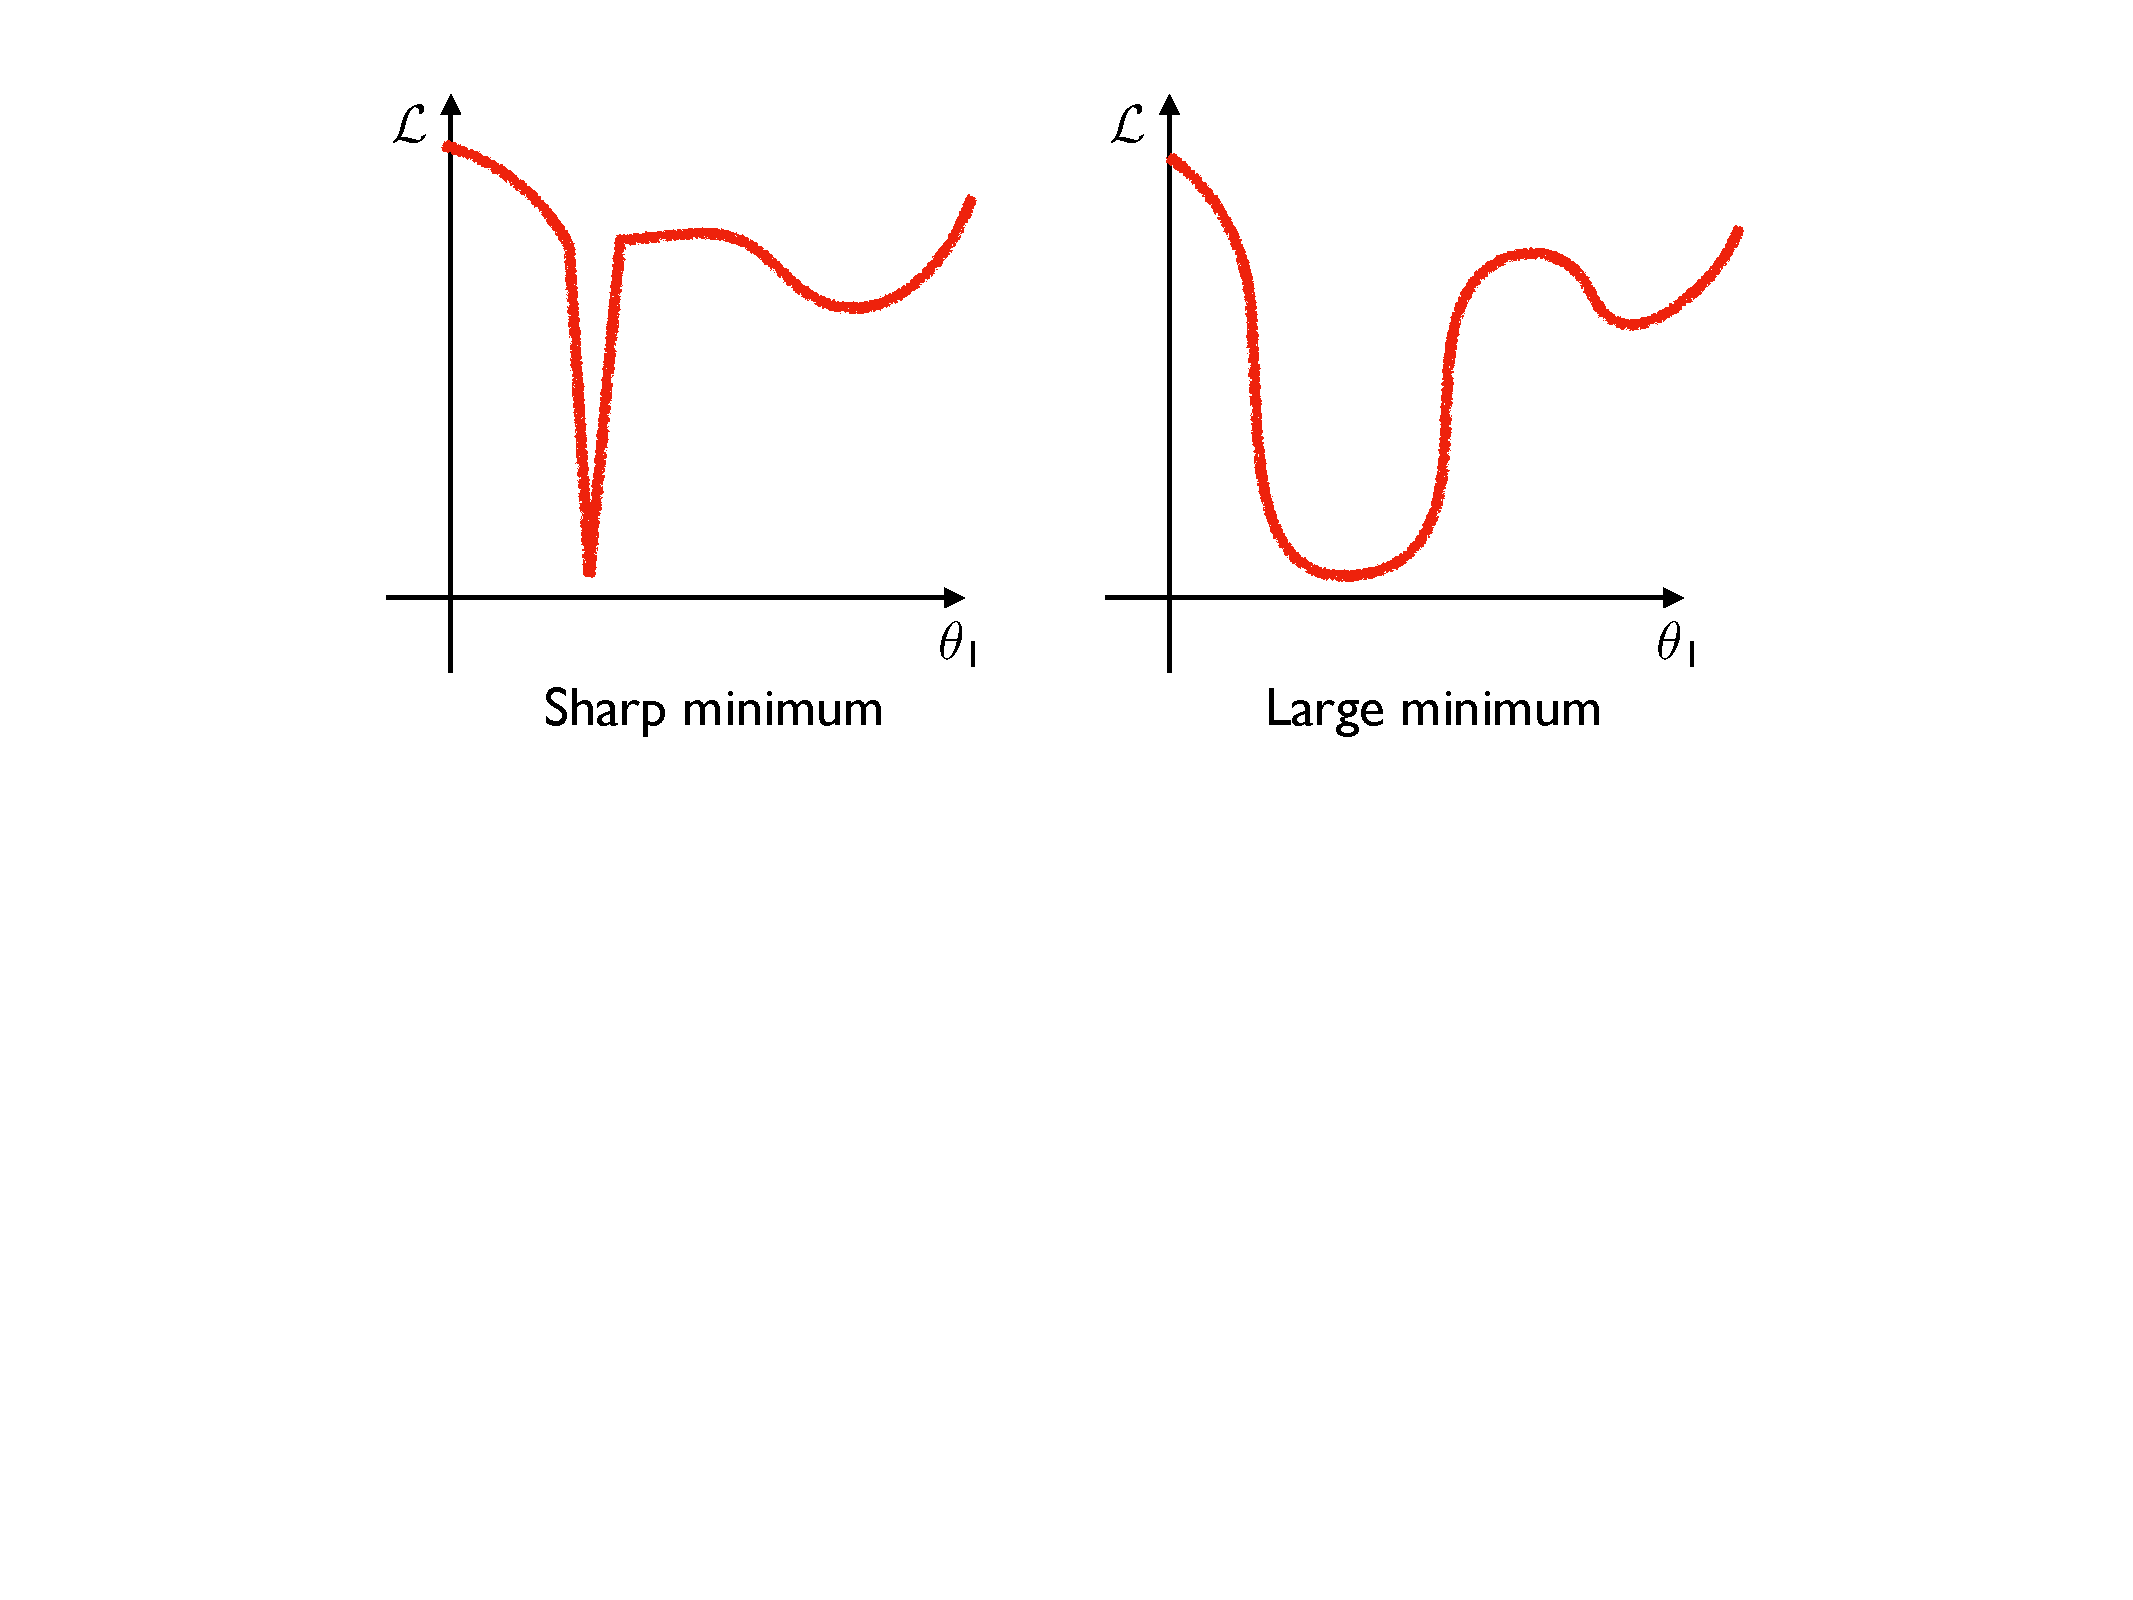
\includegraphics[width=0.9\textwidth]{../graphics/Vis_sharpness.pdf}
\end{figure}
\begin{itemize}
	\item Sharpness of a minimum: the intuition is that sharp minima are hard to find and less robust. 
	\item Scale invariance: two neural networks with ReLu as non-linearities are equivalent, if we multiply the weights of one layer with a factor and divide the weights of the next layer by the same factor. 
	\item 1D and 2D plots of the loss can therefore be misleading: the sharpness of a minimum might be due to a large extend to the problem of scale invariance. 
\end{itemize}
\end{frame}

\begin{frame}{Scale invariance and filter-wise normalization}
\begin{itemize}
	\item One idea to cope with scale invariance is to normalize the directions with respect to the filter weights \cite{Li:2018}.
	\item First we draw a random direction $d$. 
	\item We then require that the parameters belonging to the same filter $r$ in layer $l$ are normalized such that their norm is that of the filter:
	\begin{equation}
		d^l_r \leftarrow \frac{d^l_r}{\|d^l_r\|}\param^l_r
	\end{equation}
	where $\|\cdot\|$ is the Frobenius norm. 
\end{itemize}
\end{frame}

\begin{frame}{Example: effect of deeper networks}
\begin{figure}[htb]
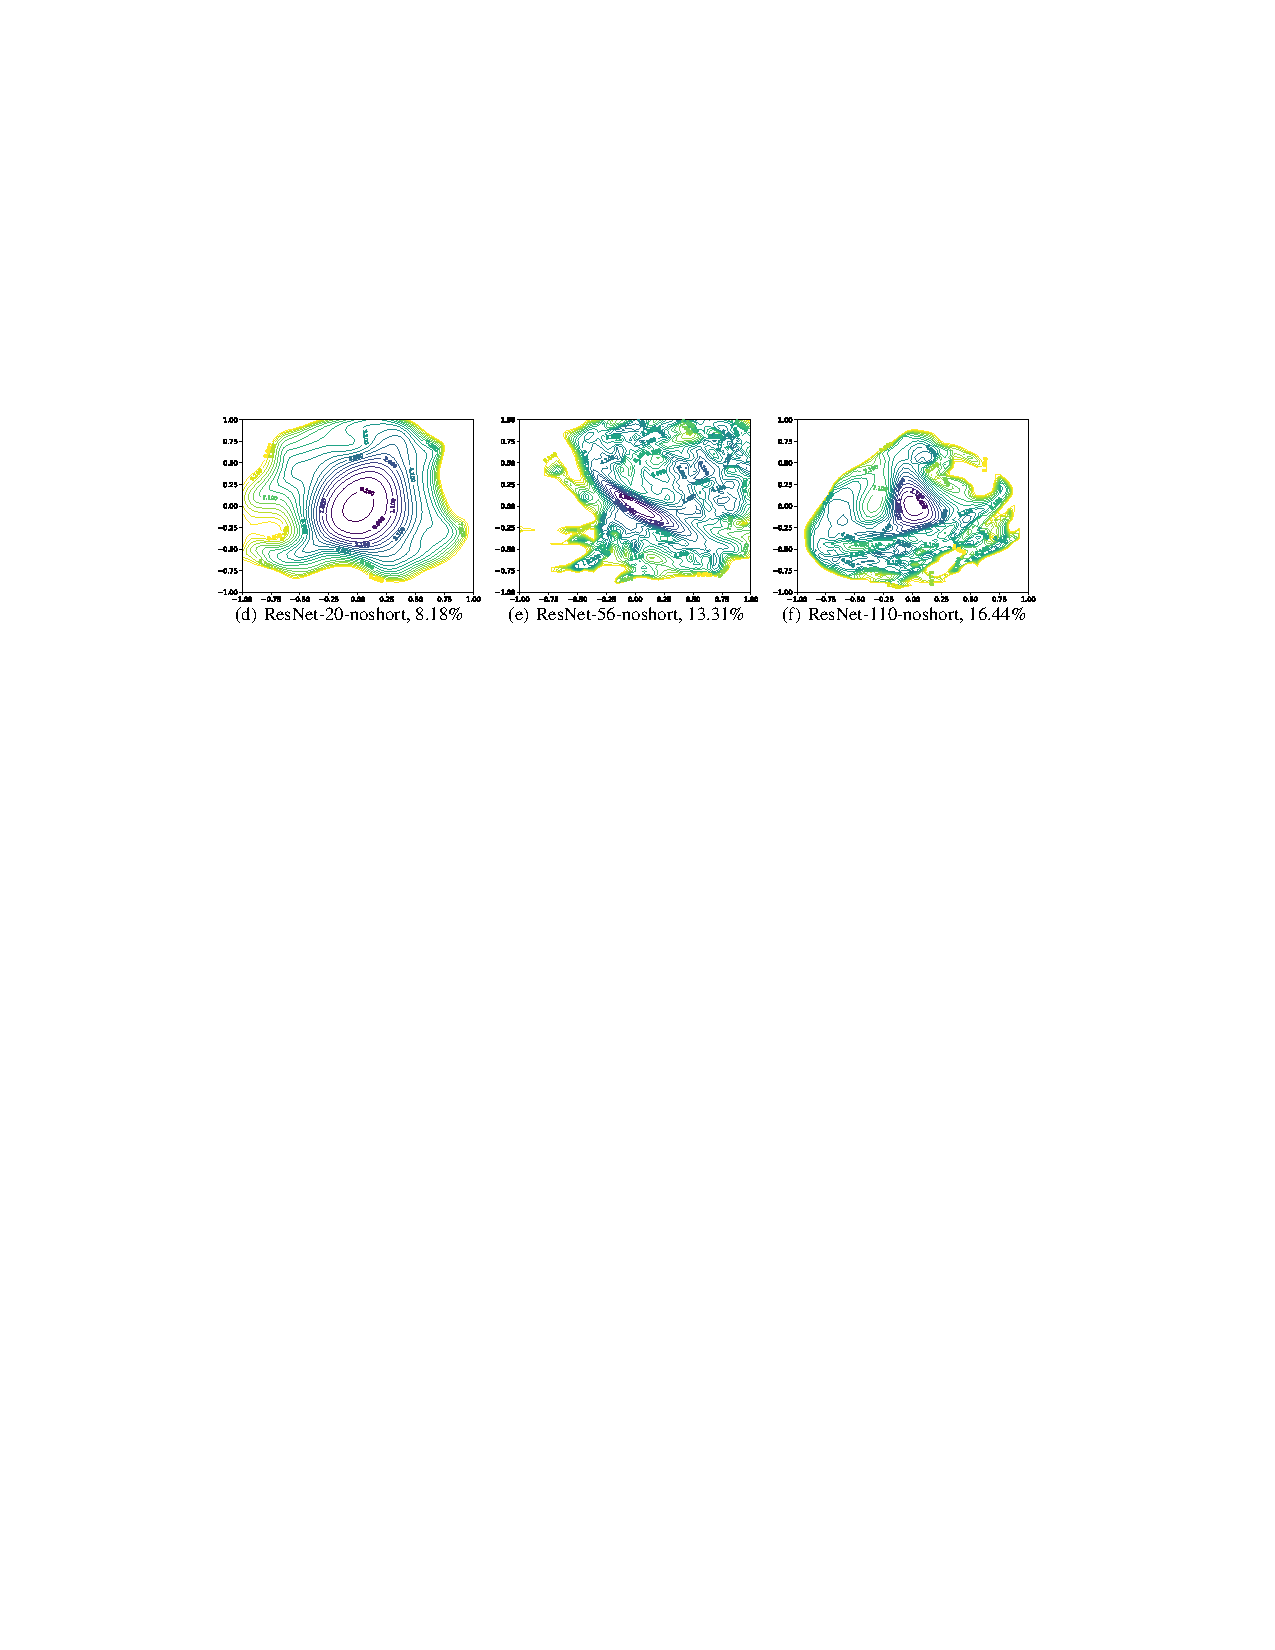
\includegraphics[width=0.9\textwidth]{../graphics/Vis_resnet_without_skip_2d.pdf}
\caption{Resnet architecture without skip connections (varying depth)}
\source{From \cite{Li:2018}}
\end{figure}
\begin{itemize}
	\item With 20 layers, we observe a fairly convex loss function. 
	\item With more layers, the loss function becomes chaotic and the gradient does not point to the global minimum. 
	\item In addition, the minima are steep and sometimes ill-conditioned (anisotropy). 
\end{itemize}
\end{frame}

\begin{frame}{Example: importance of skip-layers}
\begin{figure}[htb]
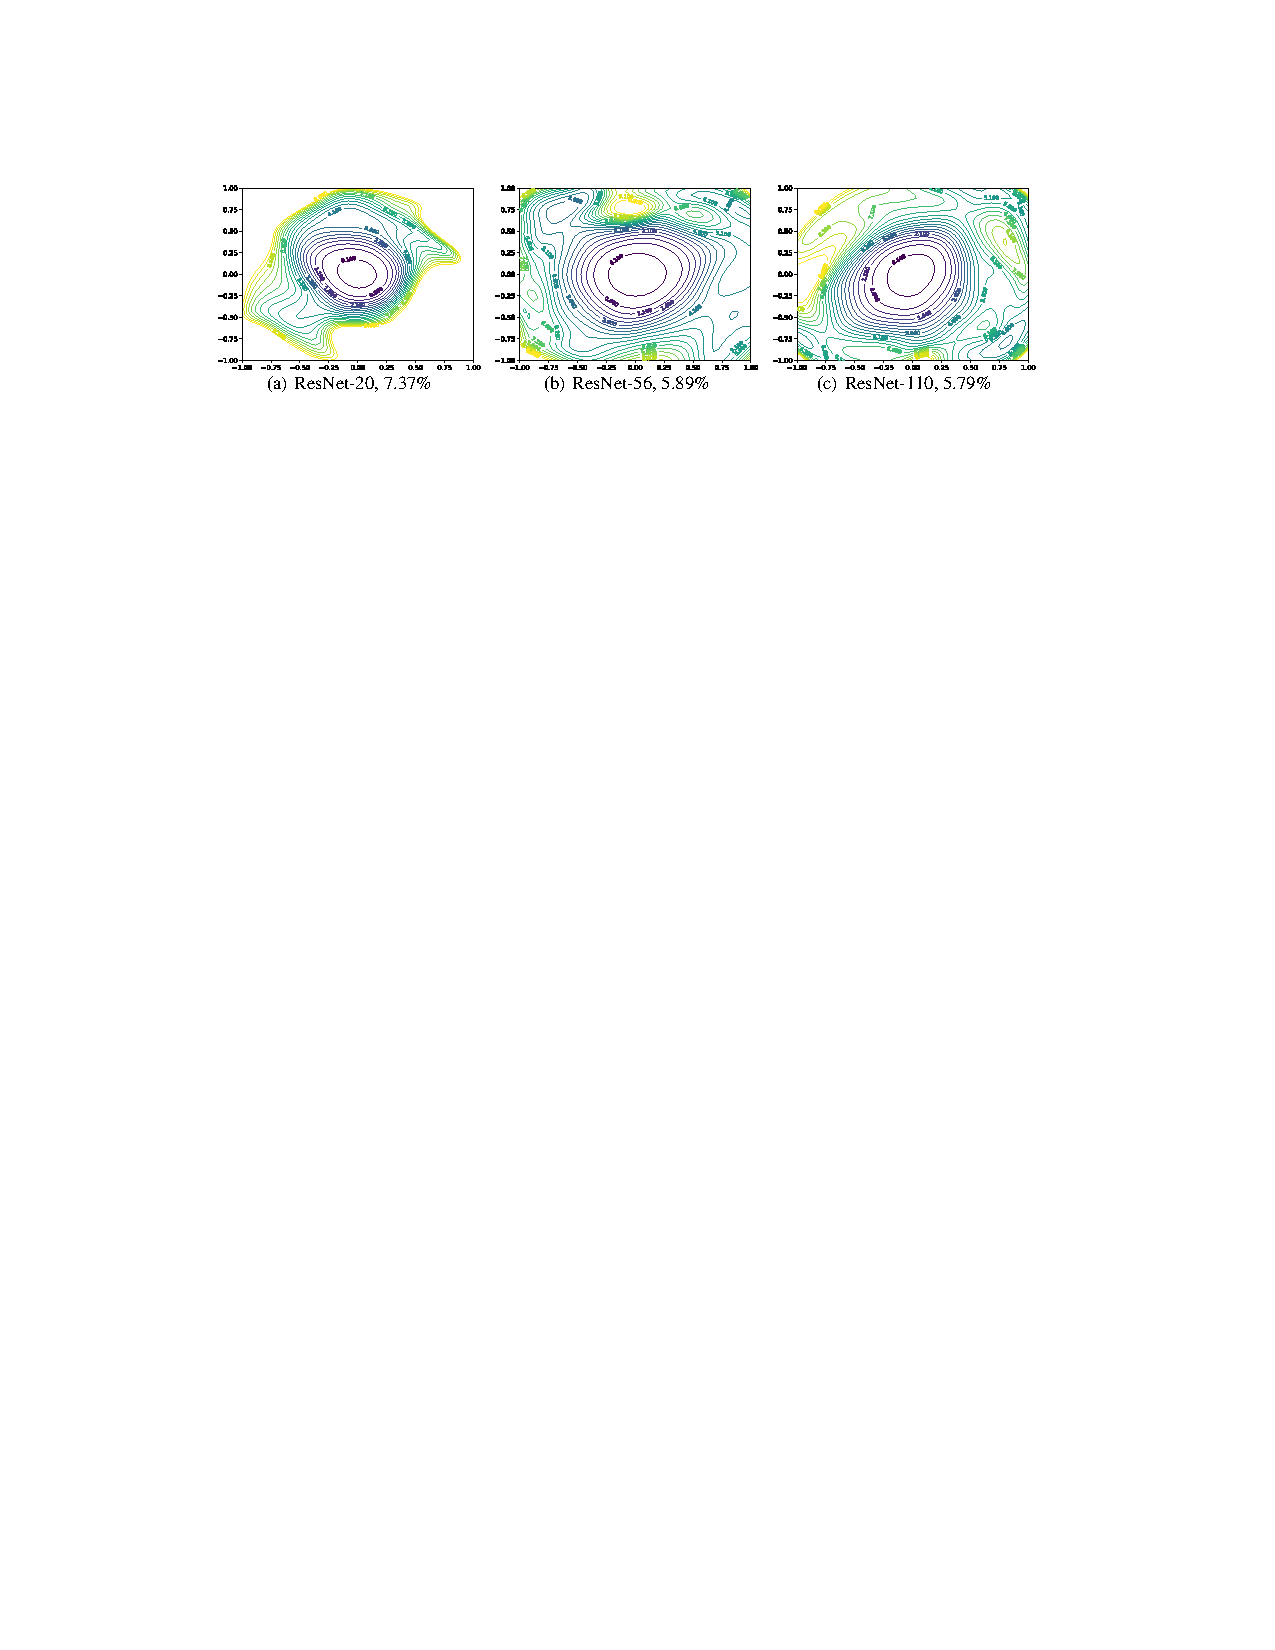
\includegraphics[width=0.9\textwidth]{../graphics/Vis_resnet_with_skip_2d.pdf}
\caption{Resnet architecture with skip connections (varying depth)}
\source{From \cite{Li:2018}}
\end{figure}
\begin{itemize}
\item Adding skip connections makes the objective function "more convex". 
\item This is particularly true for deeper networks (here: 56 and 110 layers). 
\item We therefore understand the impact of this architectural choice.
\end{itemize}
\end{frame}

\begin{frame}{More examples for the importance of skip-layers}
\begin{figure}[htb]
  \centering
  \subfloat{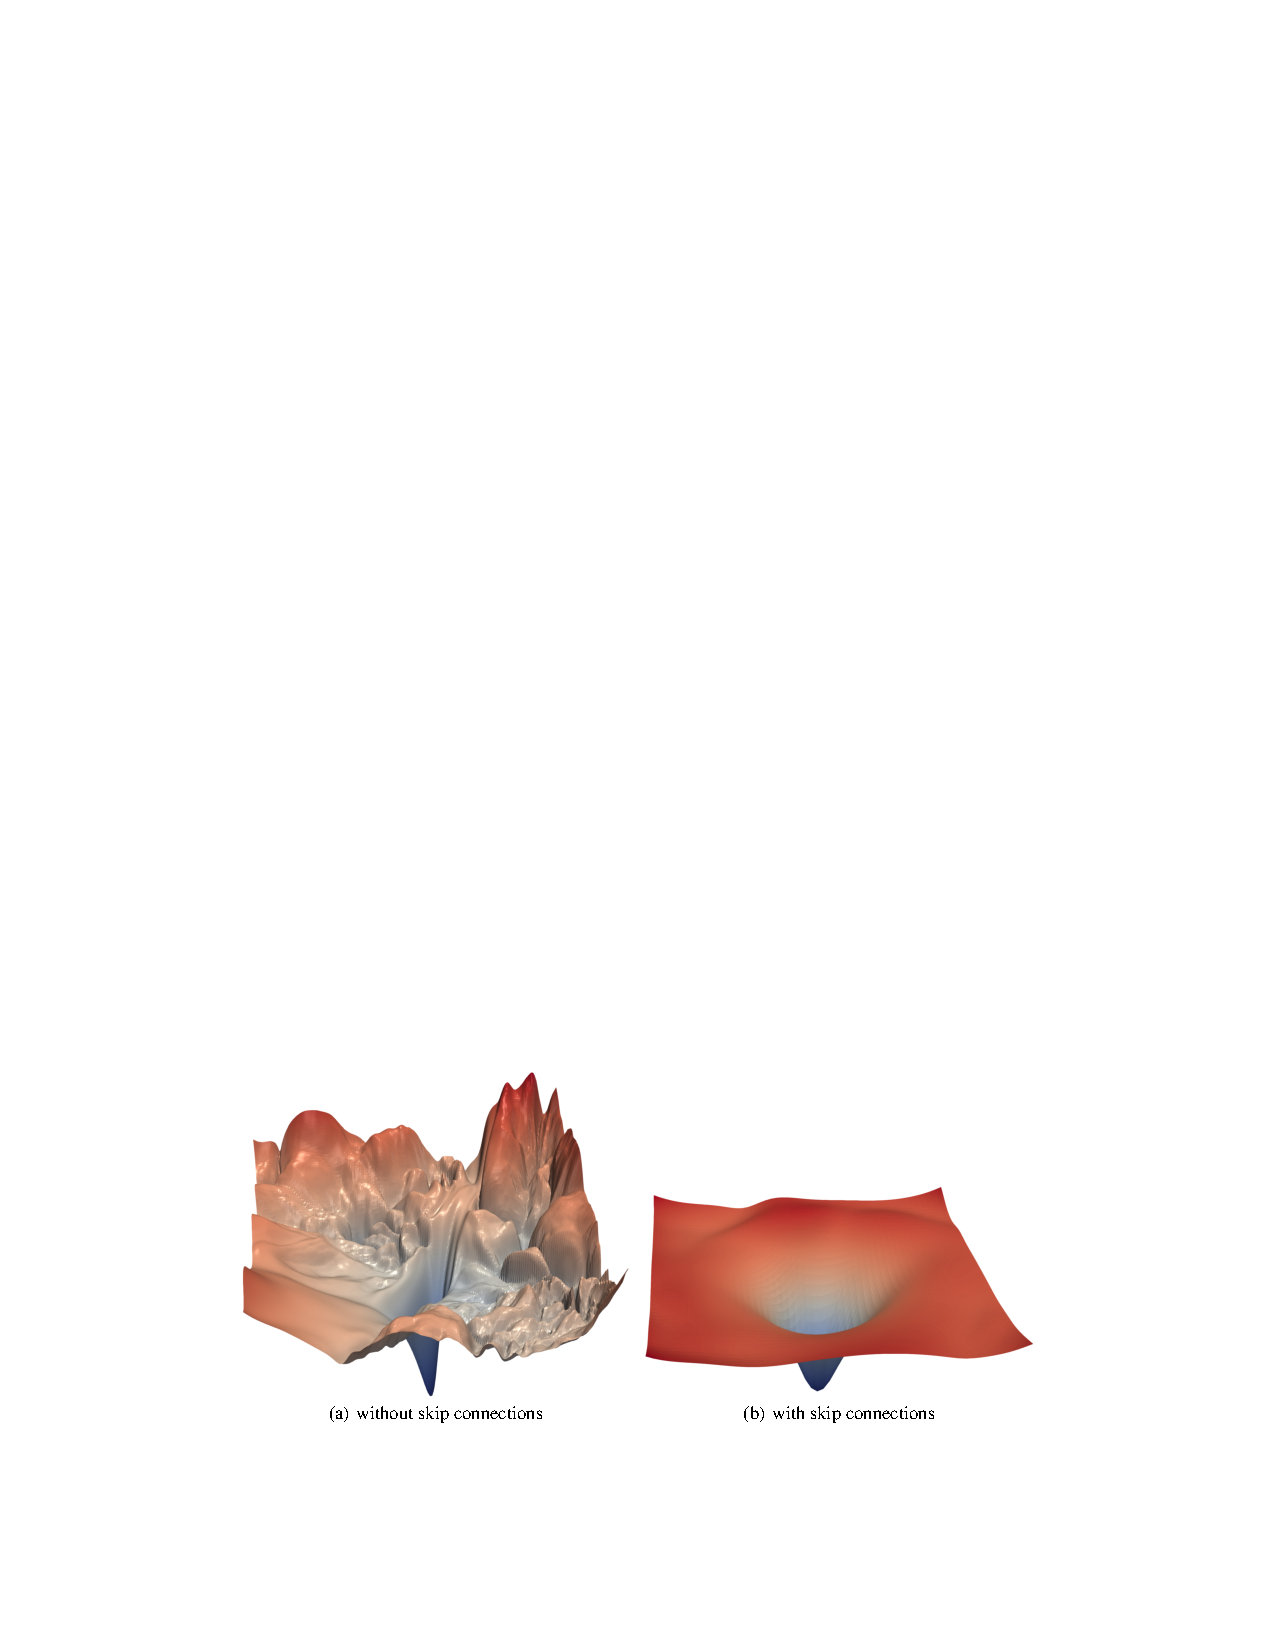
\includegraphics[width=0.7\textwidth]{../graphics/Vis_resnet_comparison_3d.pdf}}\\
  \subfloat{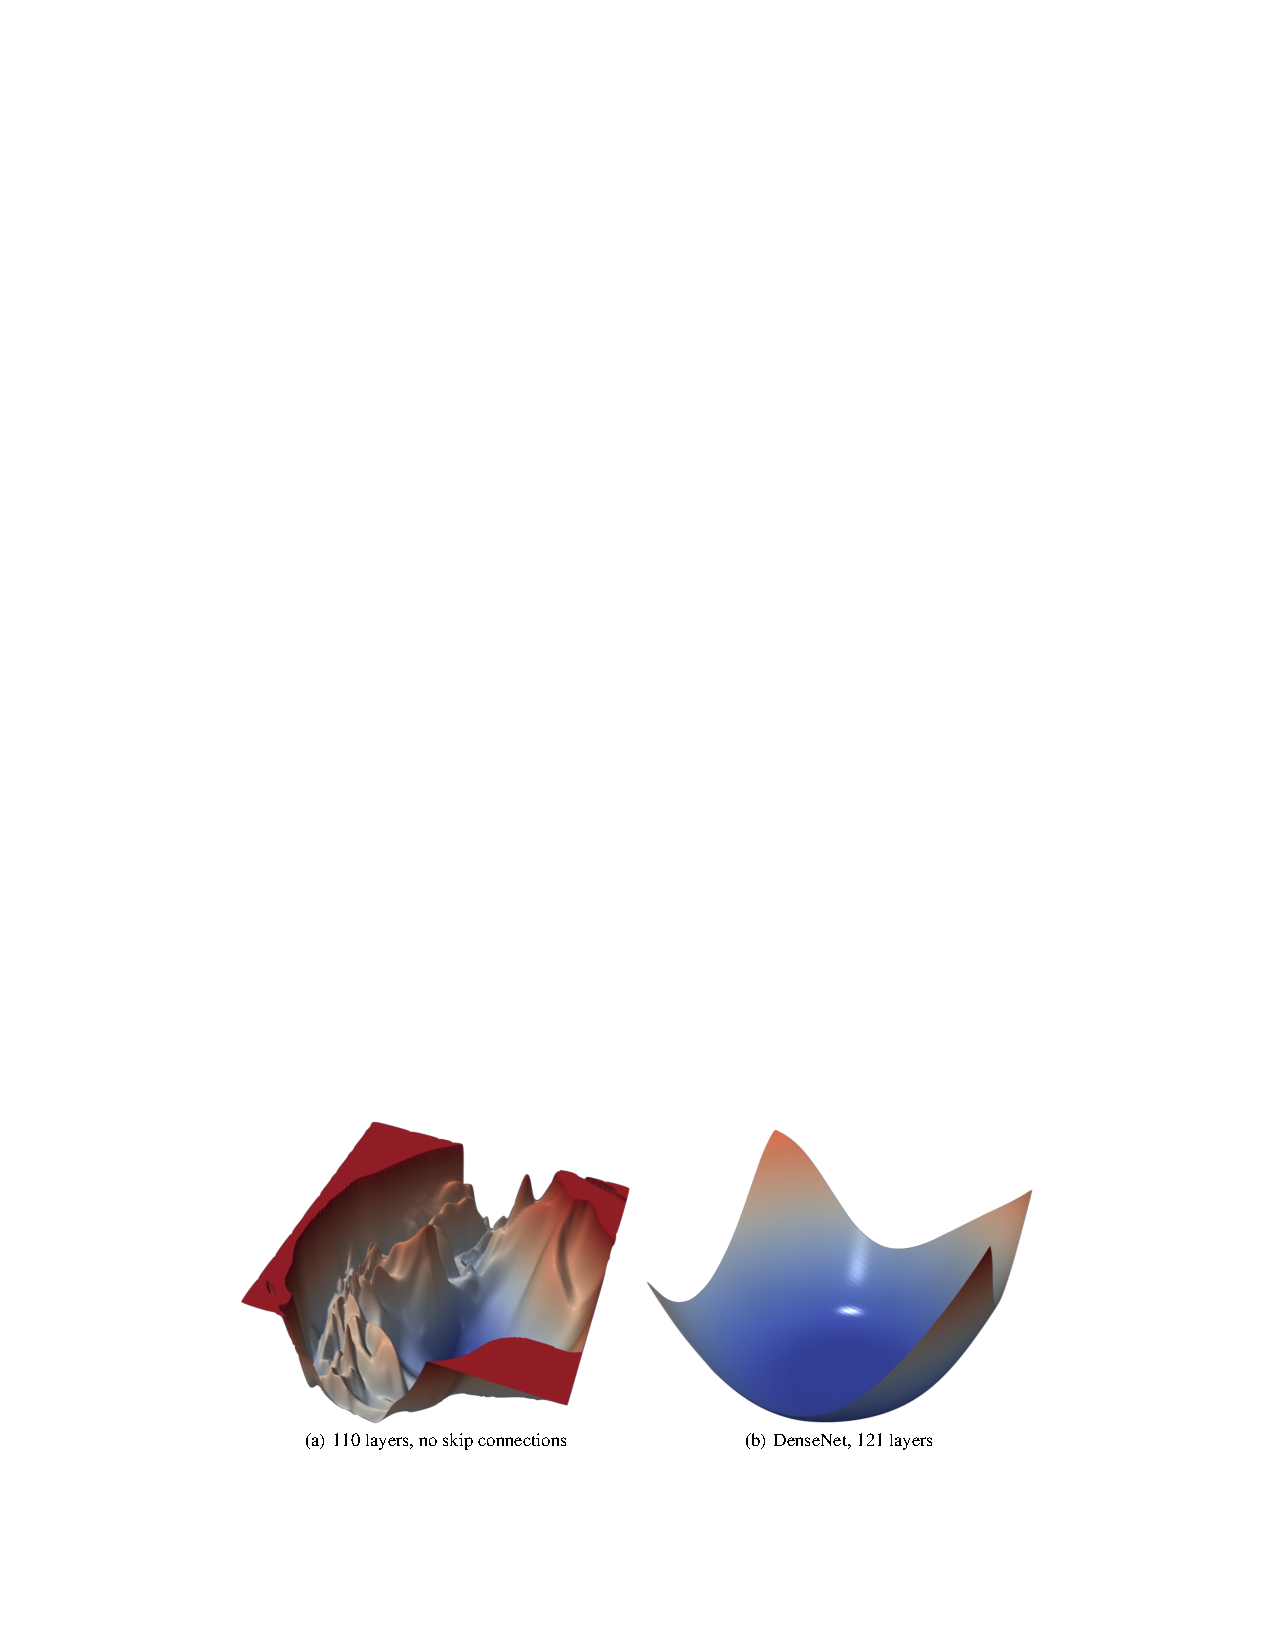
\includegraphics[width=0.7\textwidth]{../graphics/Vis_resnet_comparison2_3d.pdf}} 
  \source{From \cite{Li:2018}}
\end{figure}
\end{frame}

%%%%%%%%%%%%%%%%%%%%%%%%%%%%%%%%%%%%%%%%%%%%%%%%%%%%%%%%%%%%%%%%%%%%%%%%%
%%%%%%%%%%%%%%%%%%%%%%%%%%%%%%%%%%%%%%%%%%%%%%%%%%%%%%%%%%%%%%%%%%%%%%%%%
\section{References}
\begin{frame}[allowframebreaks]
	\frametitle{References}
	\bibliography{slides_deep.bib}
\end{frame}


\end{document}